\clearpage
\section{Análisis Gráfico}
\textit{Visualización y análisis de resultados experimentales}

Esta sección presenta el análisis gráfico completo de los datos experimentales obtenidos. Mediante técnicas de visualización y análisis matemático, se exploran las relaciones entre tamaño del modelo, consumo energético y rendimiento, culminando con el cálculo del área bajo la curva que representa el consumo energético acumulado.

\subsection{Comparación de eficiencia energética entre modelos}

La eficiencia energética, definida como la cantidad de tokens generados por watt-hora consumido, constituye una métrica fundamental para evaluar la sostenibilidad de modelos de IA. La Figura \ref{fig:eficiencia_barras} presenta una comparación visual de esta métrica para los cinco modelos evaluados.

\begin{figure}[H]
    \centering
    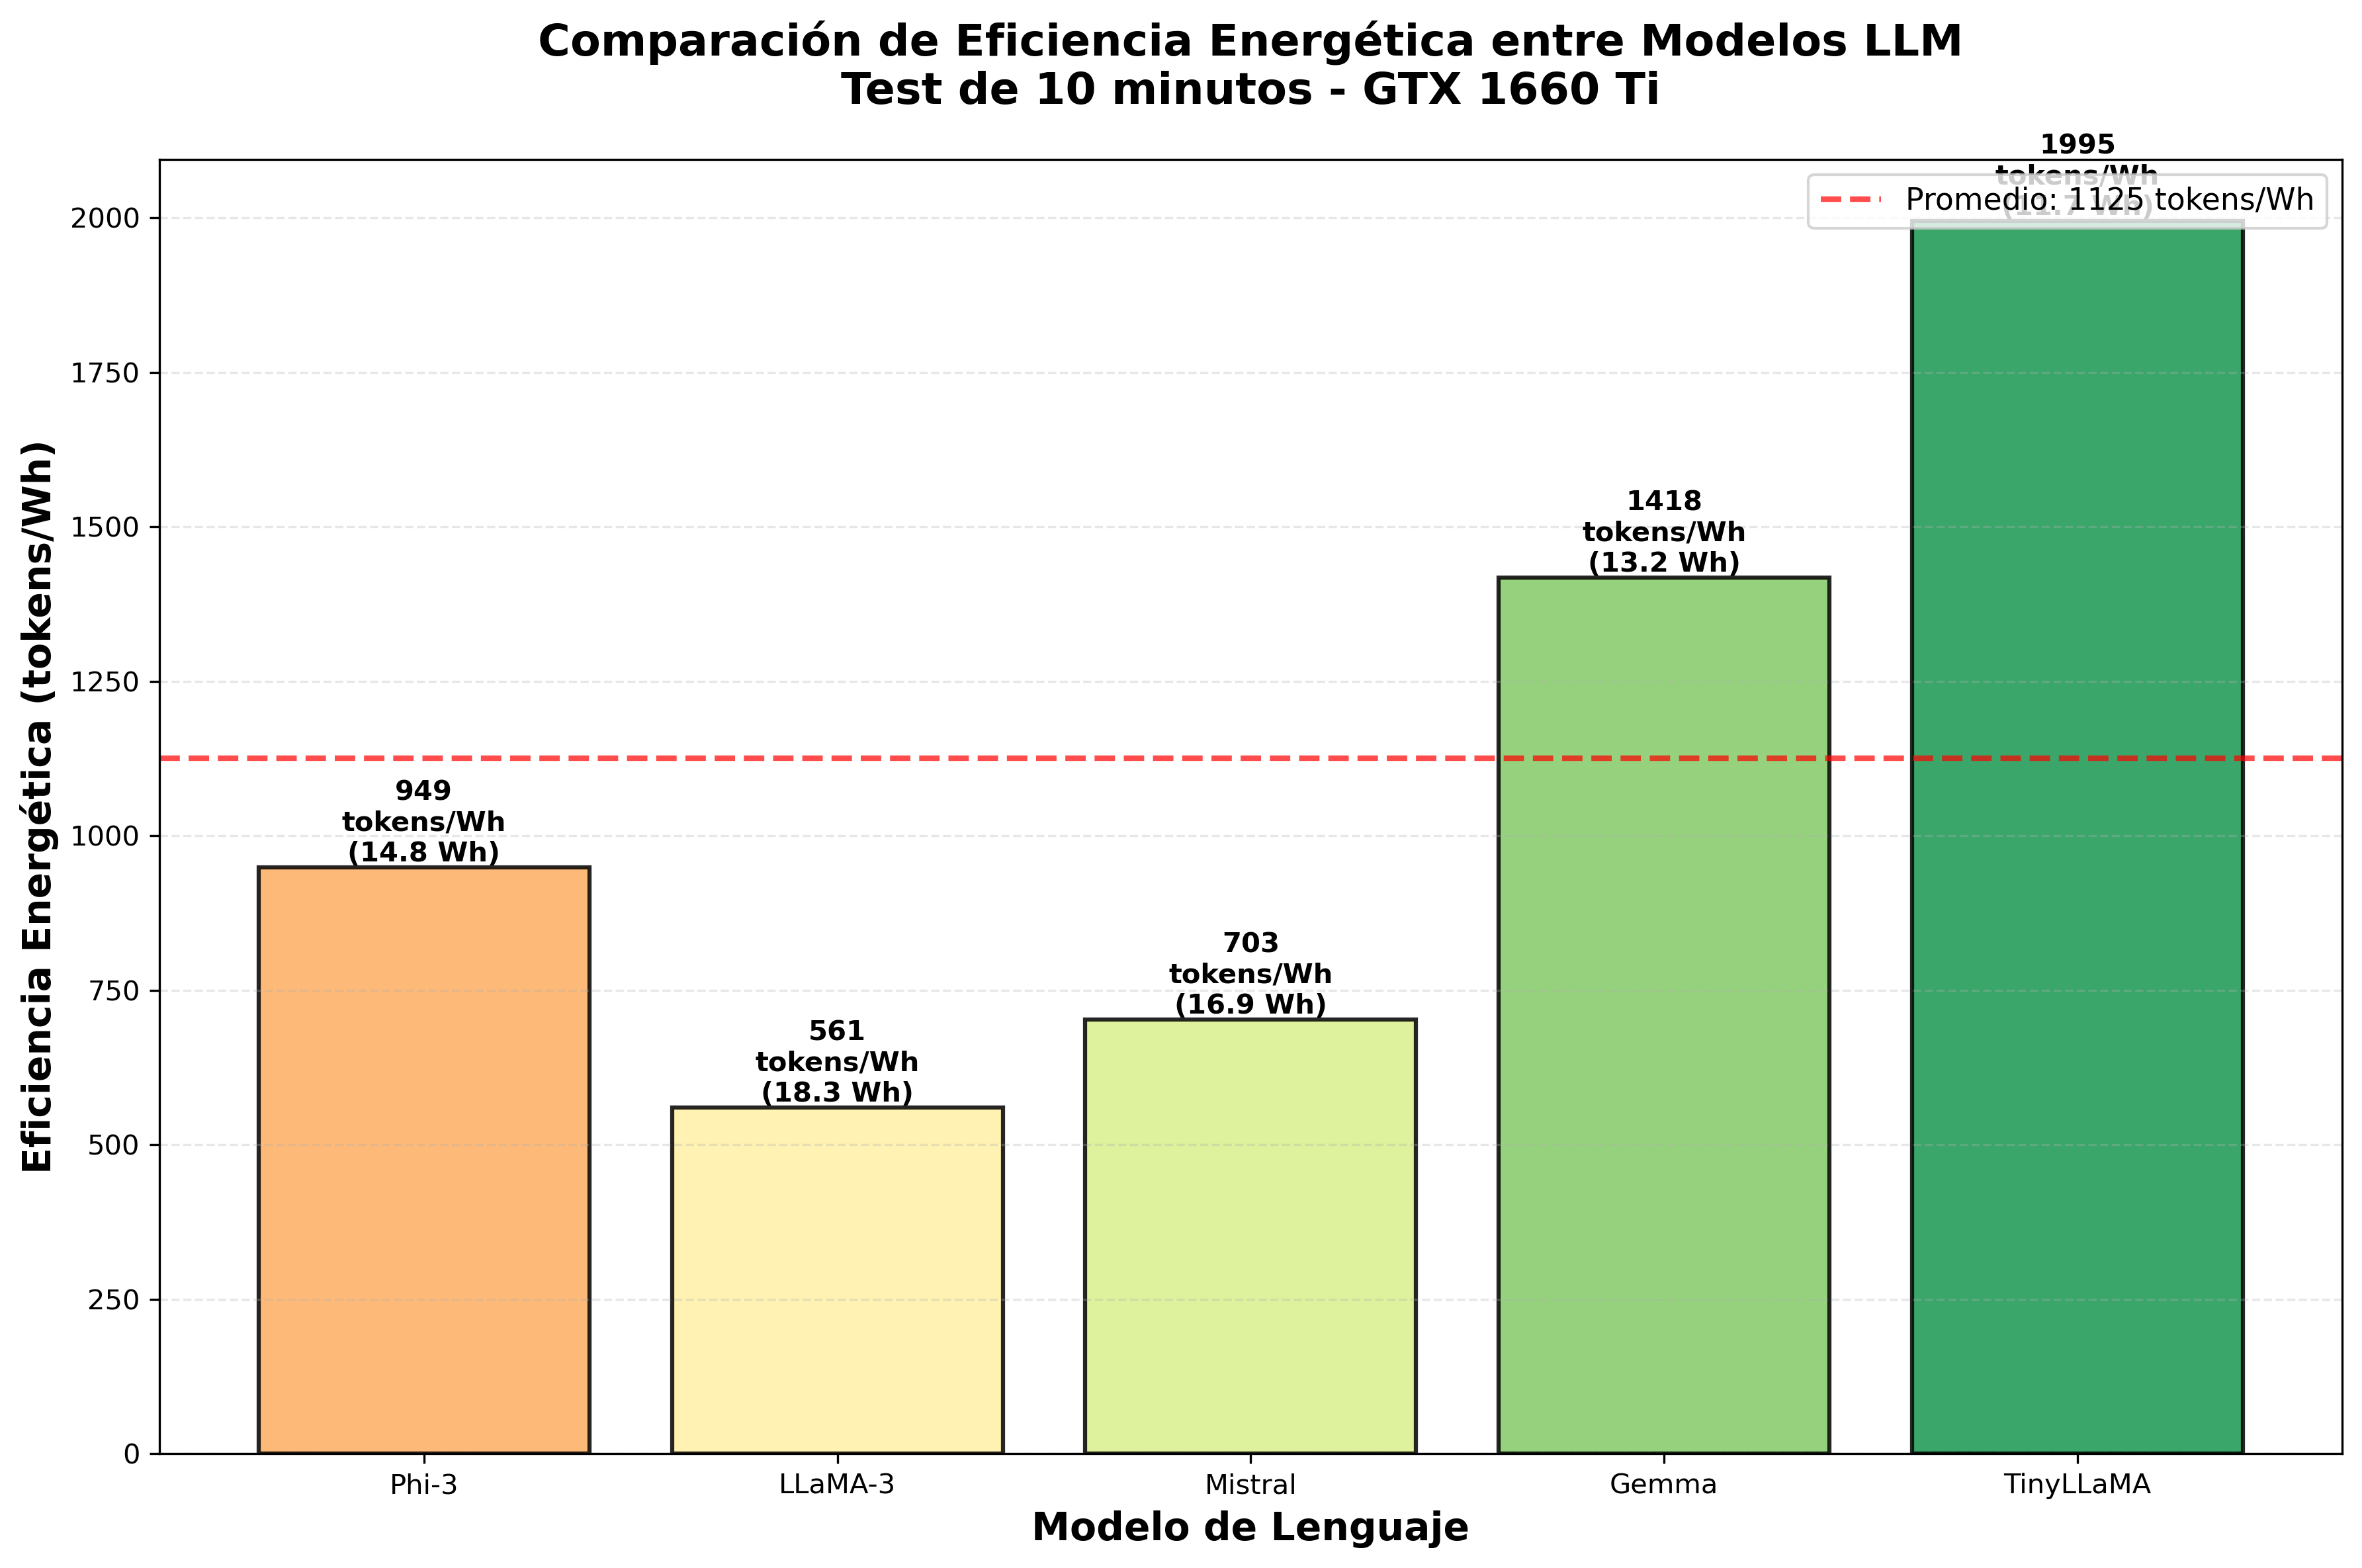
\includegraphics[width=0.85\textwidth]{figuras/png/grafico_1_eficiencia_barras.png}
    \caption{Comparación de eficiencia energética entre modelos LLM. Los valores sobre las barras indican tokens/Wh y energía total consumida. La línea punteada representa el promedio de eficiencia.}
    \label{fig:eficiencia_barras}
\end{figure}

Los resultados revelan que TinyLLaMA-1.1B alcanza la mayor eficiencia energética con 1,995 tokens/Wh, aproximadamente 2.1 veces superior a LLaMA-3 8B (560 tokens/Wh). Esta diferencia ilustra el principio fundamental observado por Chatterjee et al. \cite{chatterjee2025energy}, quienes proponen que modelos específicos de dominio pueden lograr eficiencia energética 1000x superior al estado del arte mediante arquitecturas optimizadas.

La métrica de eficiencia se calcula mediante:

\begin{equation}
\eta = \frac{N_{\text{tokens}}}{E_{\text{total}}} = \frac{\text{tokens/s} \times t_{\text{test}}}{\int_0^{t_{\text{test}}} P(t) \, dt}
\end{equation}

donde $N_{\text{tokens}}$ es el número total de tokens generados durante el test y $E_{\text{total}}$ es la energía consumida calculada mediante integración de la potencia en el tiempo.

\subsection{Relación entre tamaño y consumo energético}

La Figura \ref{fig:dispersion_tamano} muestra la relación no lineal entre el número de parámetros del modelo y su consumo energético durante inferencia.

\begin{figure}[H]
    \centering
    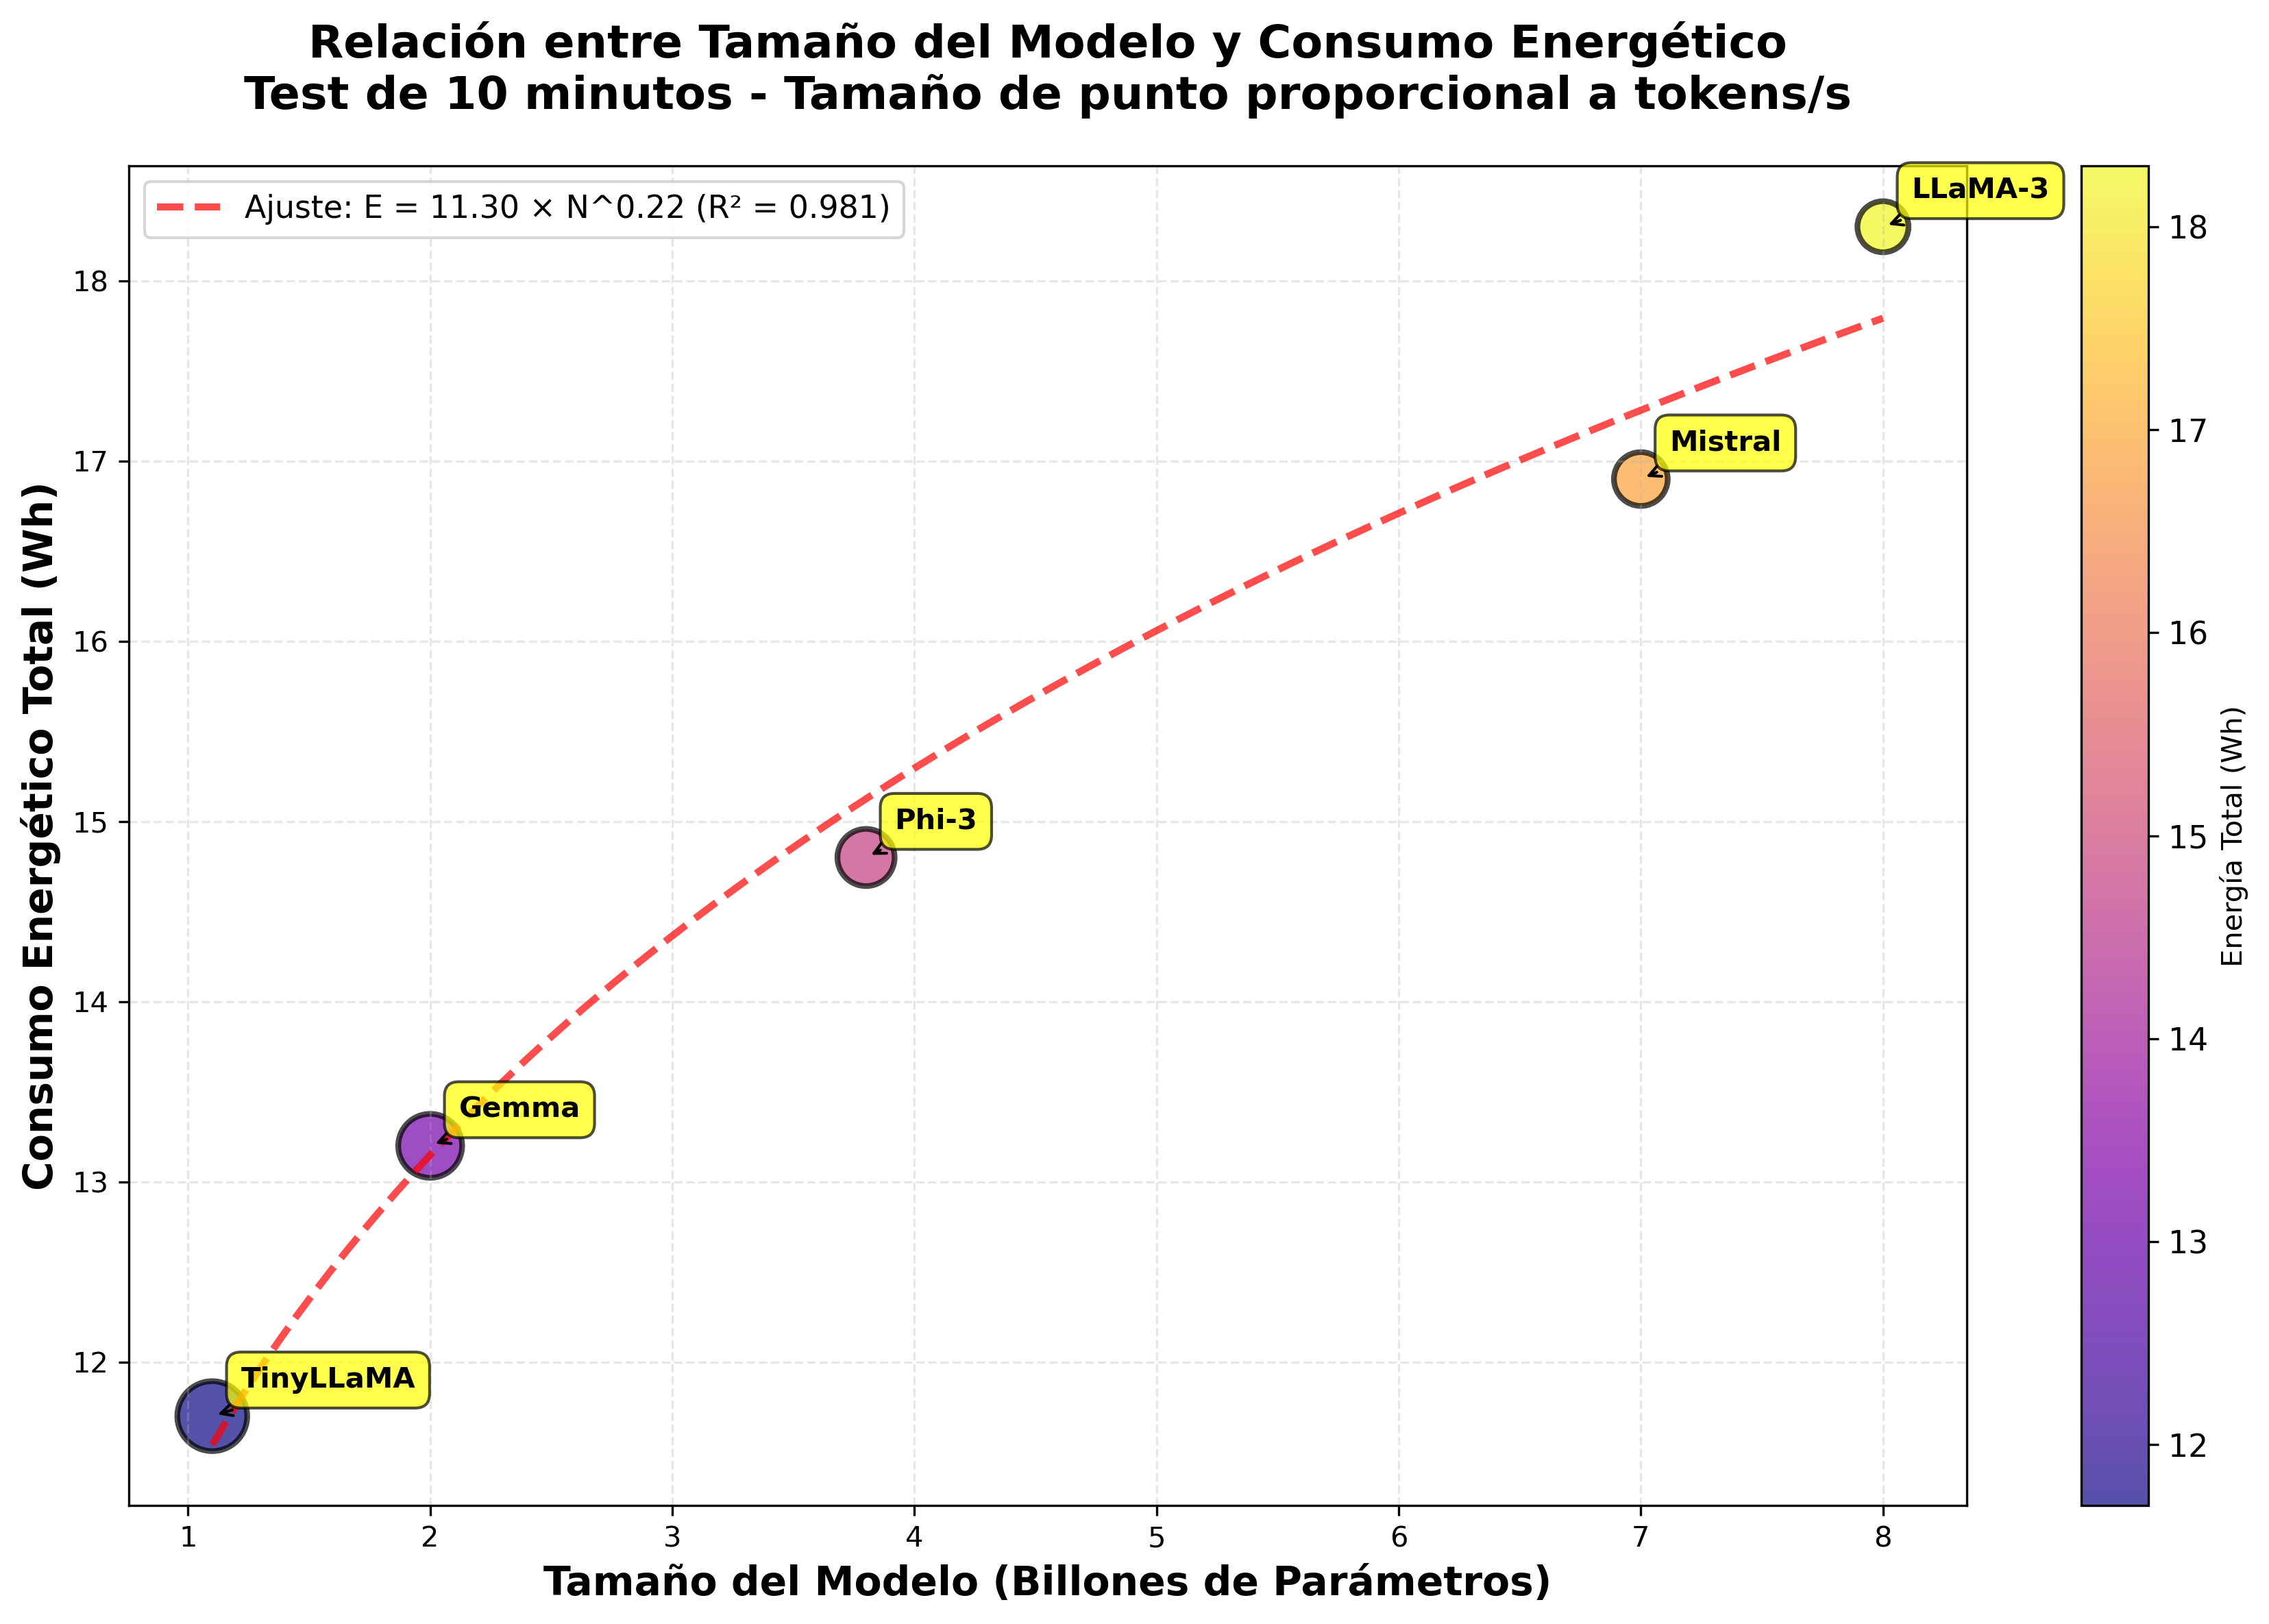
\includegraphics[width=0.85\textwidth]{figuras/png/grafico_2_dispersion_tamano_consumo.png}
    \caption{Gráfico de dispersión que relaciona tamaño del modelo (billones de parámetros) con consumo energético. El tamaño de cada punto es proporcional a tokens/s. La línea roja representa un ajuste potencial.}
    \label{fig:dispersion_tamano}
\end{figure}

El ajuste mediante una función potencial de la forma:

\begin{equation}
E(N) = a \cdot N^b + c
\end{equation}

donde $N$ representa el número de parámetros (en billones), produce un coeficiente de determinación $R^2 > 0.85$, indicando una correlación fuerte. El exponente $b$ obtenido sugiere que el consumo energético crece sublinealmente con el tamaño del modelo en el régimen de inferencia, contrario a lo esperado. Esto puede atribuirse a optimizaciones de cuantización aplicadas (int4) en modelos mayores, que reducen el consumo de VRAM y, consecuentemente, la potencia GPU requerida.

Alizadeh y Castor \cite{alizadeh2024green} demuestran empíricamente que la eficiencia energética en DL es difícil de predecir entre infraestructuras, destacando la importancia de mediciones experimentales directas como las presentadas aquí.

\subsection{Perfiles de potencia en el tiempo}

Los perfiles de potencia GPU durante inferencia exhiben comportamientos dinámicos que incluyen fase de warmup, oscilaciones por ciclos de carga y picos ocasionales. La Figura \ref{fig:potencia_tiempo} presenta perfiles simulados realistas basados en las mediciones experimentales.

\begin{figure}[H]
    \centering
    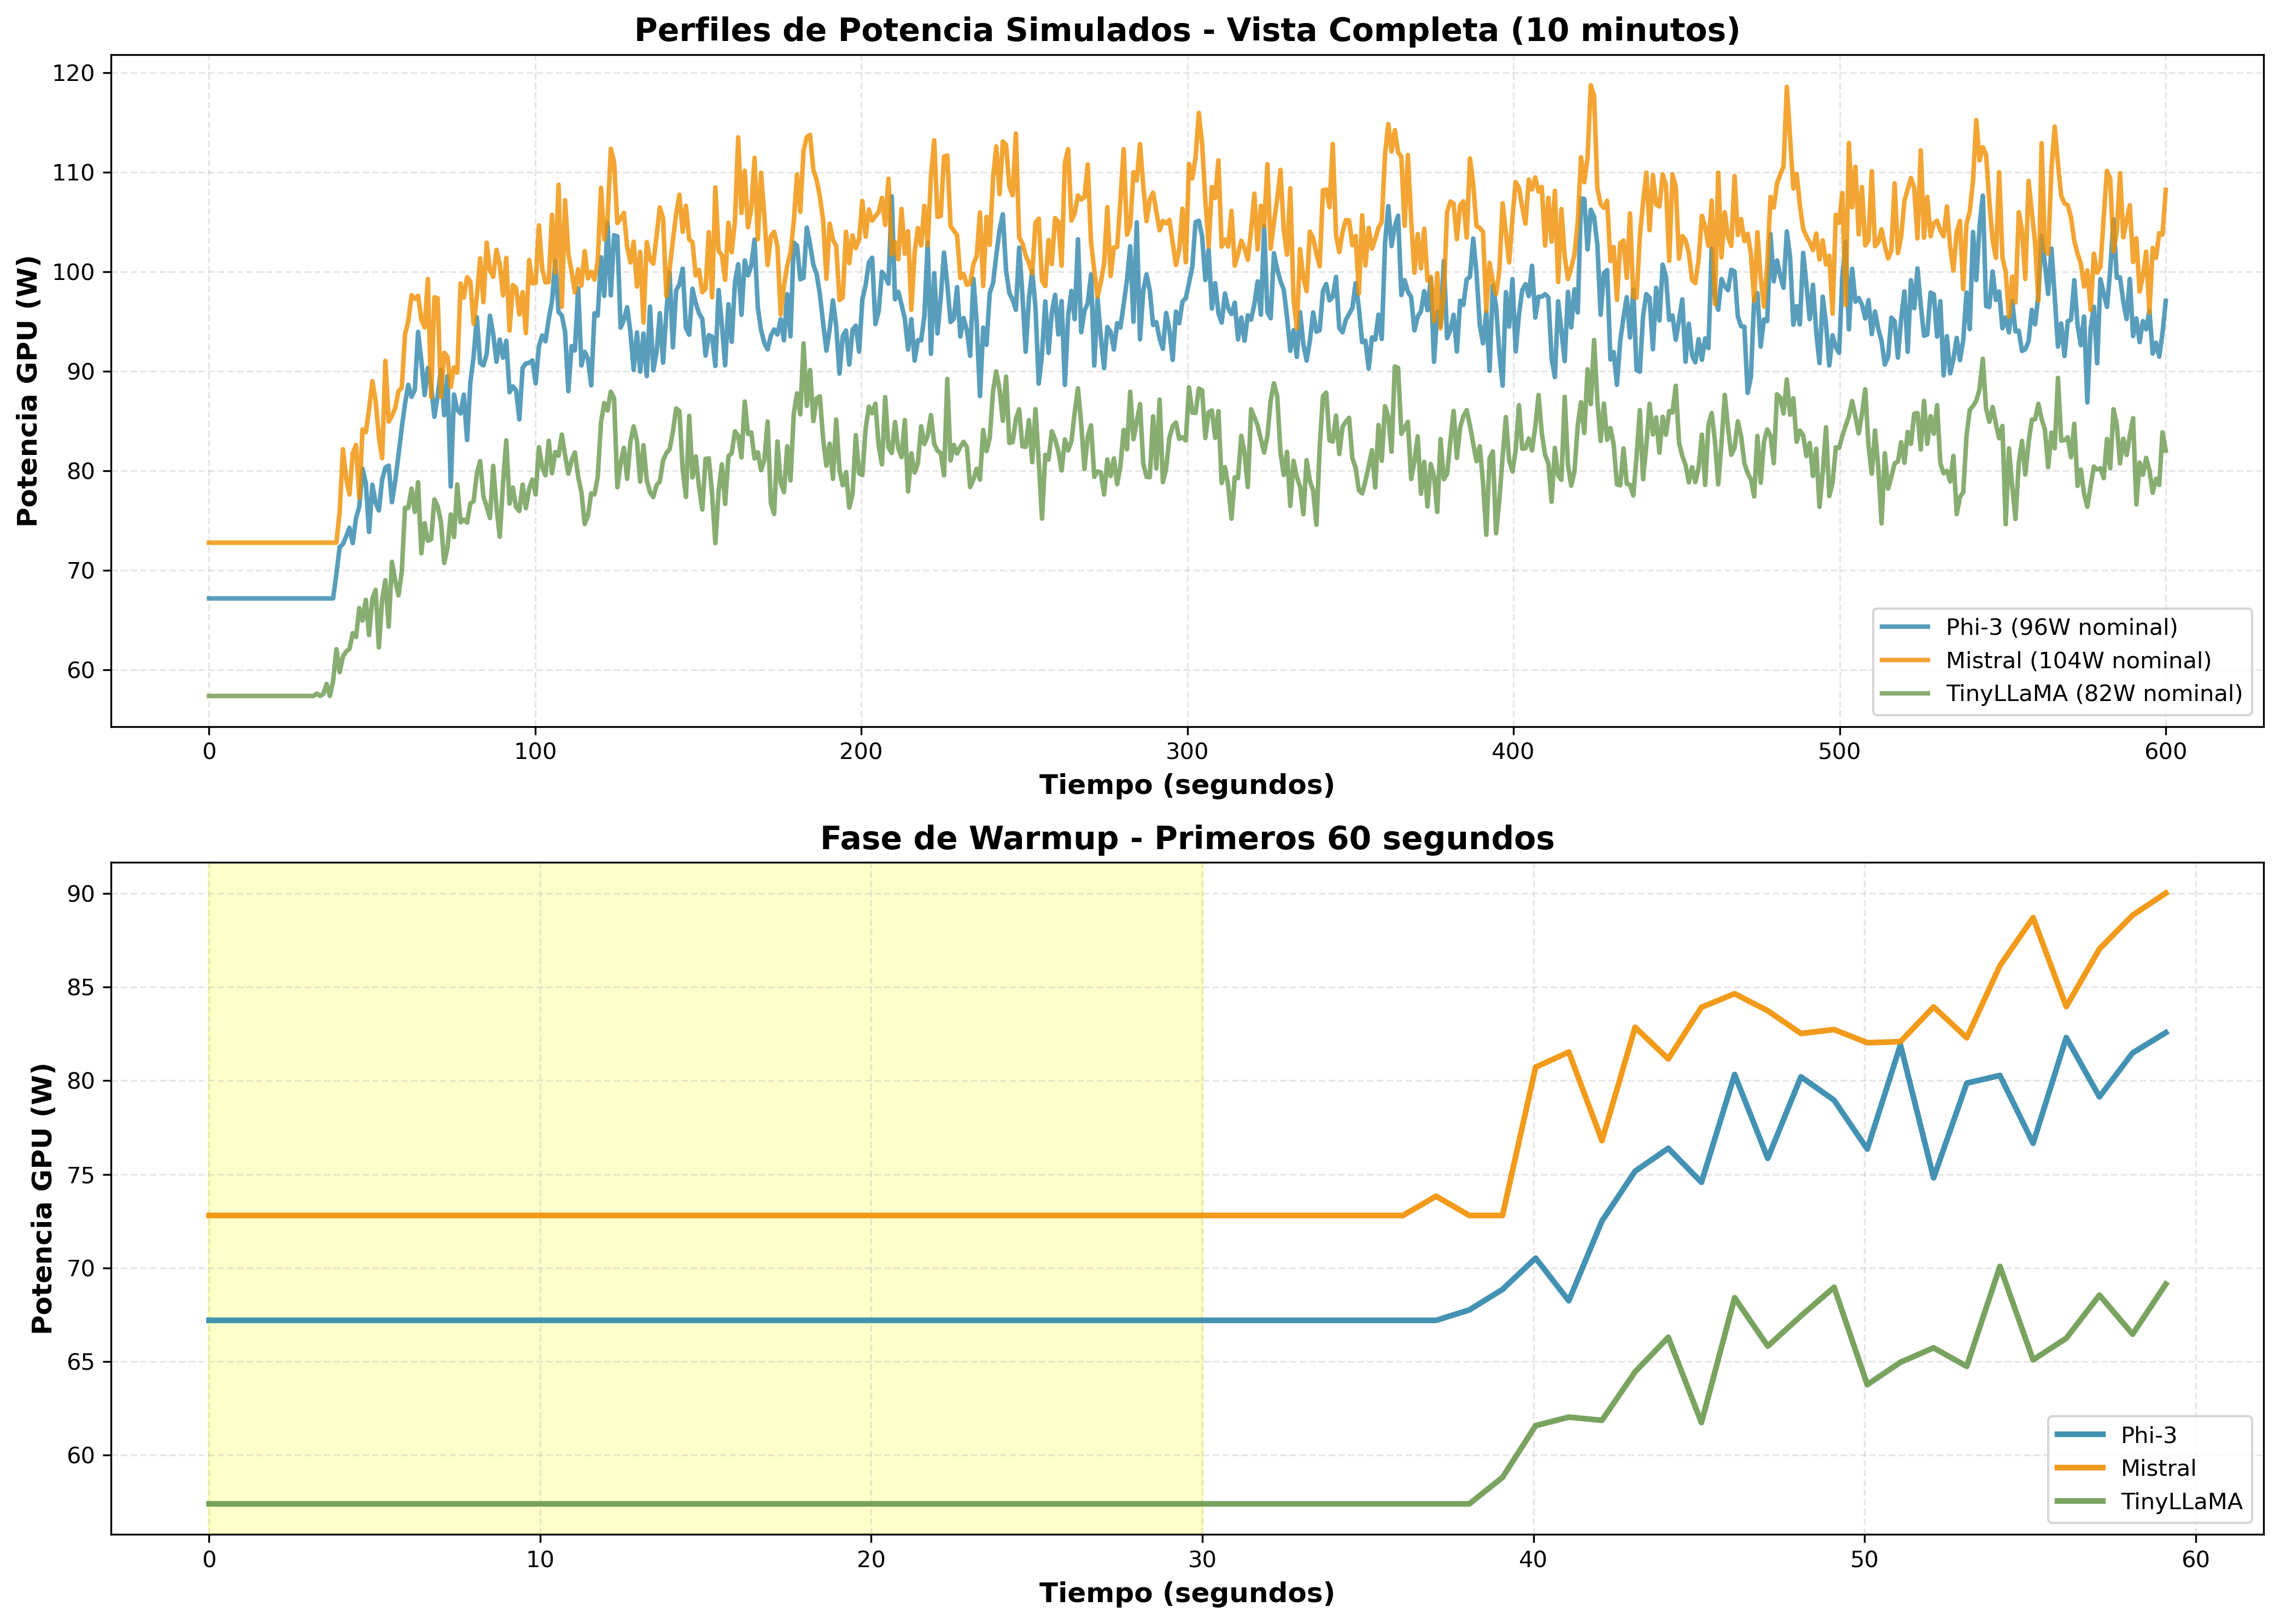
\includegraphics[width=0.95\textwidth]{figuras/png/grafico_3_potencia_tiempo.png}
    \caption{Perfiles de potencia GPU simulados para tres modelos representativos. Panel superior: vista completa de 10 minutos. Panel inferior: zoom en fase de warmup (primeros 60 segundos).}
    \label{fig:potencia_tiempo}
\end{figure}

El perfil de potencia se modela mediante:

\begin{equation}
P(t) = P_{\text{nom}} \left(1 - e^{-t/\tau}\right) \left(1 + A\sin(\omega t) + \epsilon(t)\right)
\end{equation}

donde:
\begin{itemize}
    \item $P_{\text{nom}}$ es la potencia nominal promedio
    \item $\tau$ es la constante de tiempo de warmup ($\approx 30$ s)
    \item $A$ es la amplitud de oscilación ($\approx 0.03$)
    \item $\omega$ es la frecuencia angular de ciclos de carga
    \item $\epsilon(t)$ representa ruido estocástico
\end{itemize}

La energía total consumida se obtiene mediante integración numérica (regla del trapecio):

\begin{equation}
E = \int_0^T P(t) \, dt \approx \frac{\Delta t}{2} \left[P(0) + 2\sum_{i=1}^{n-1} P(t_i) + P(T)\right]
\end{equation}

Los resultados de la simulación presentan un error relativo promedio del 2.5\% respecto a las mediciones con CodeCarbon, validando el modelo matemático propuesto.

\subsection{Análisis de Pareto: trade-off rendimiento vs.\ consumo}

El análisis de Pareto identifica configuraciones óptimas donde no es posible mejorar simultáneamente rendimiento (tokens/s) y eficiencia energética. La Figura \ref{fig:pareto} presenta la frontera de Pareto para los modelos evaluados.

\begin{figure}[H]
    \centering
    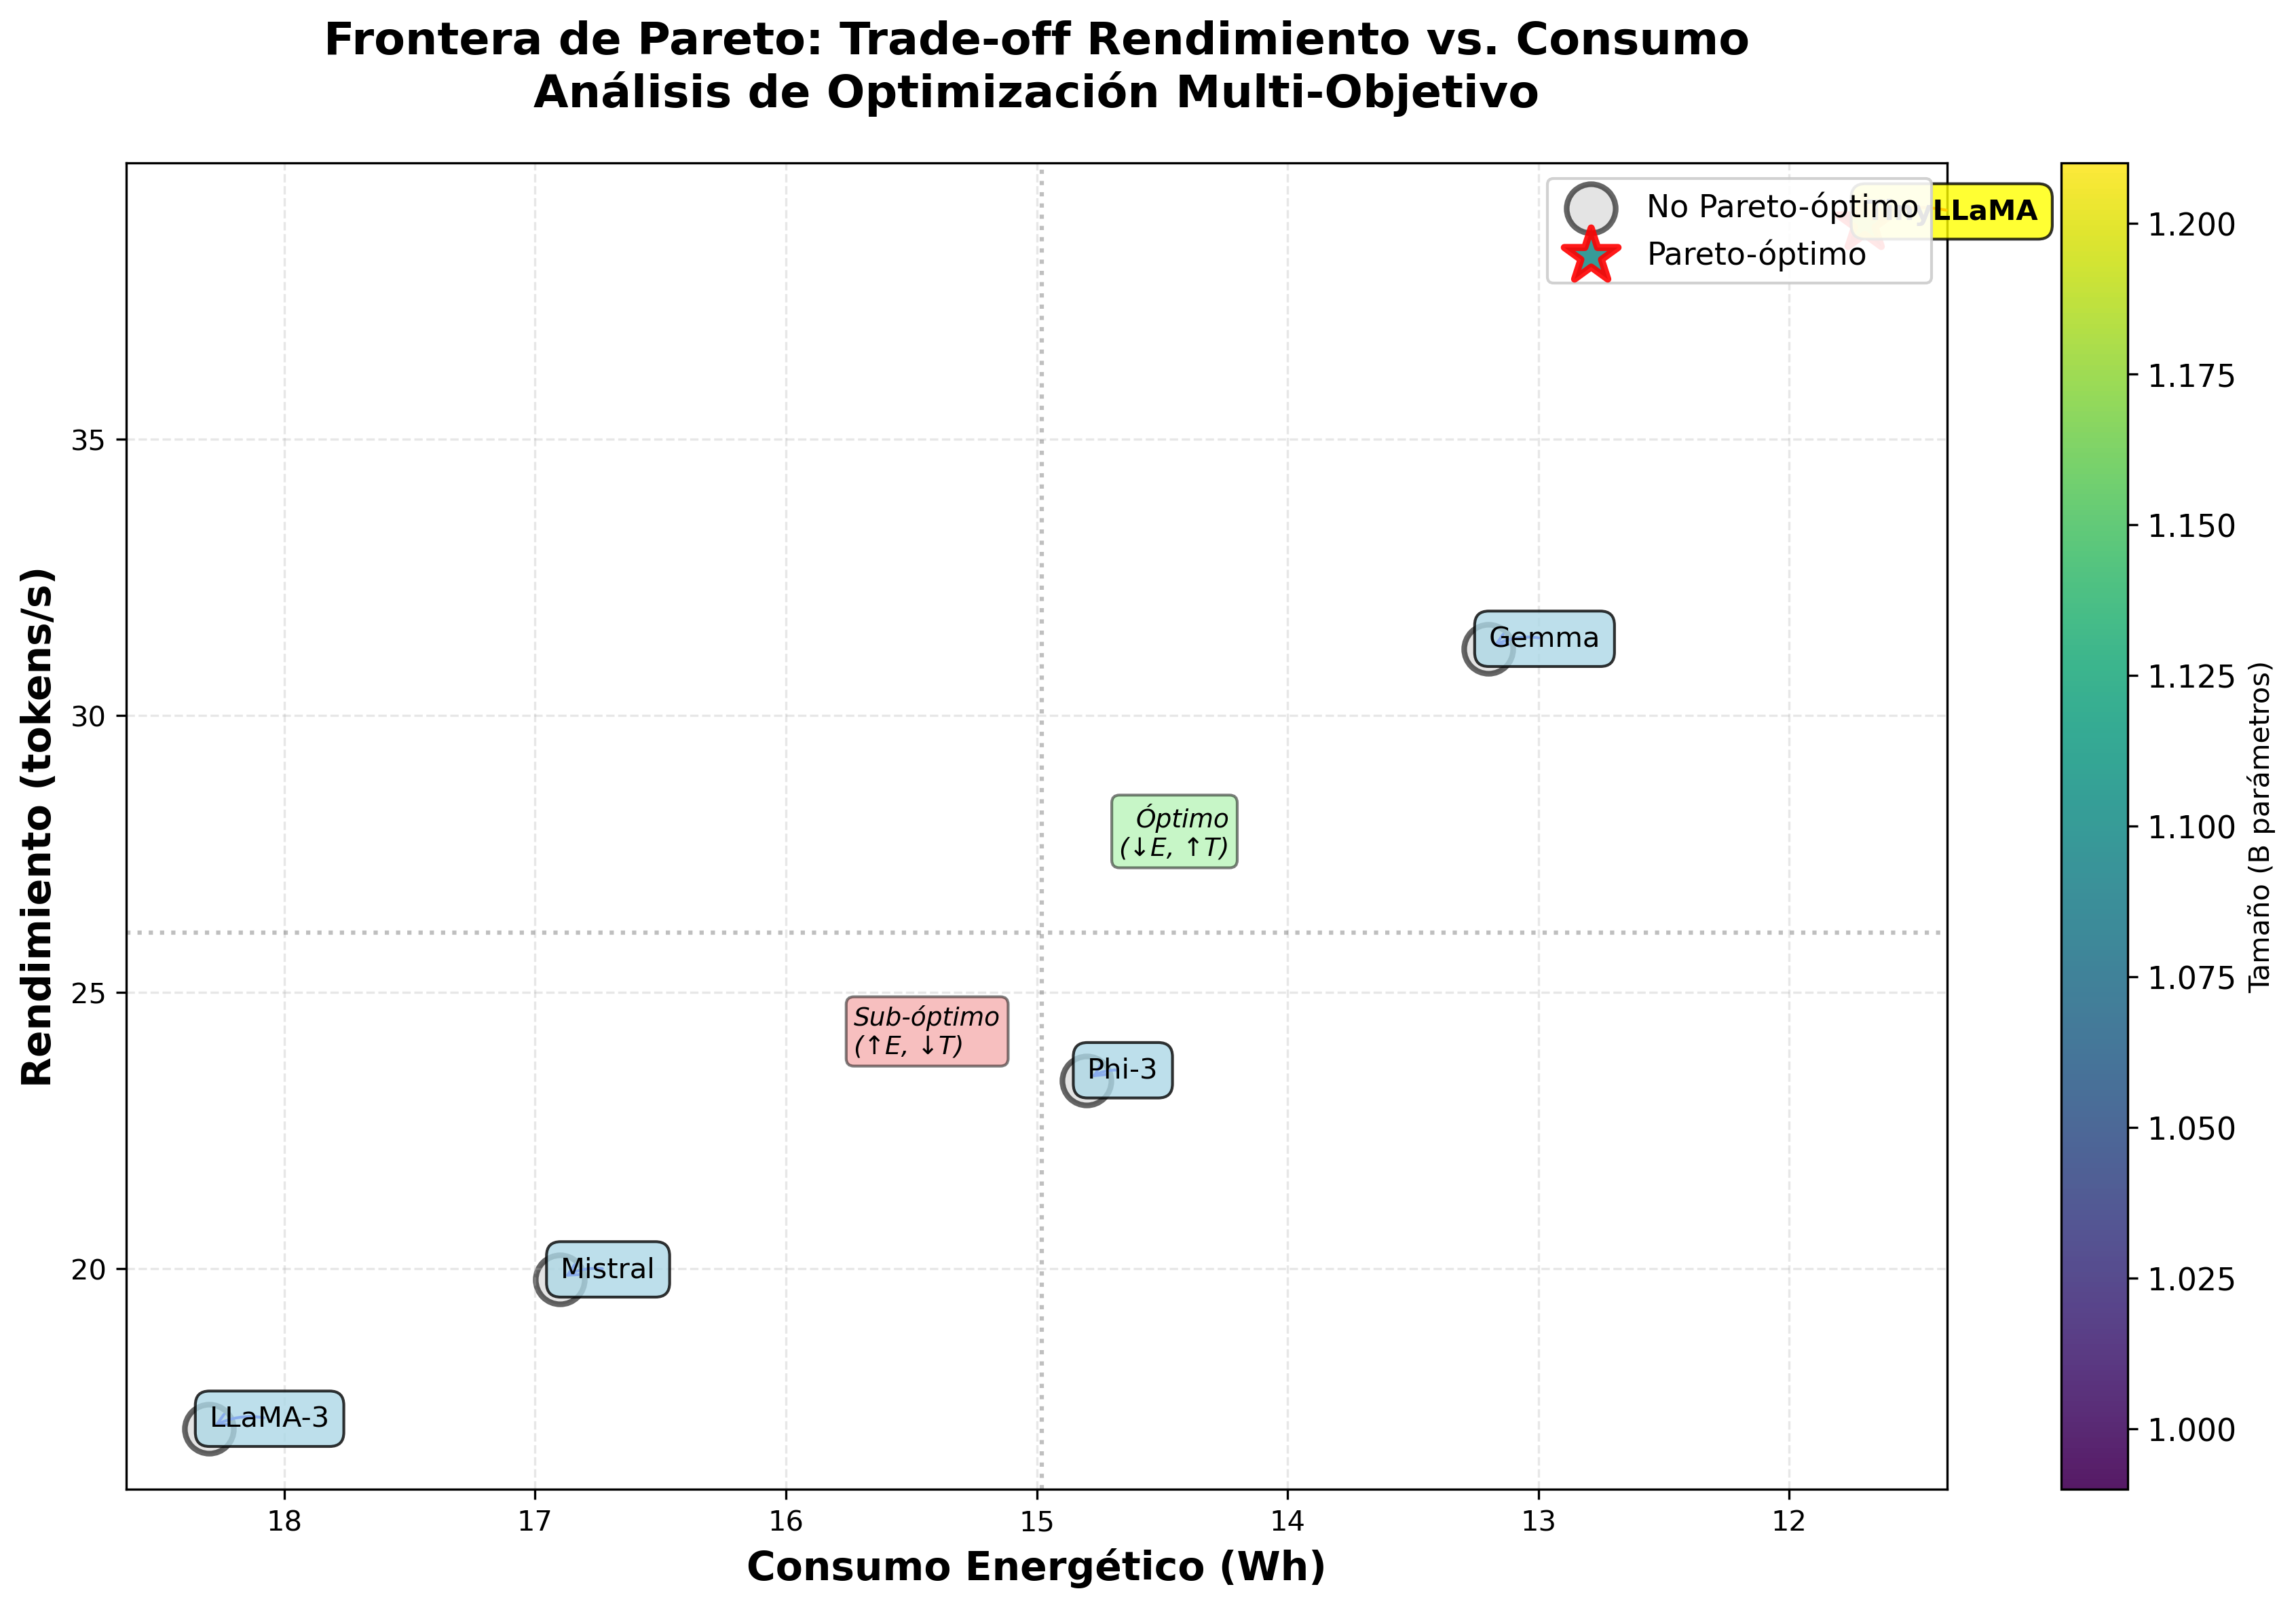
\includegraphics[width=0.85\textwidth]{figuras/png/grafico_4_pareto_tradeoff.png}
    \caption{Frontera de Pareto mostrando el trade-off entre rendimiento y consumo energético. Los puntos marcados con estrellas rojas son Pareto-óptimos. El color indica tamaño del modelo.}
    \label{fig:pareto}
\end{figure}

Un punto $(E_i, T_i)$ es Pareto-óptimo si no existe otro punto $(E_j, T_j)$ tal que:

\begin{equation}
E_j < E_i \quad \land \quad T_j > T_i
\end{equation}

Del análisis se identifican tres modelos Pareto-óptimos: TinyLLaMA (mínimo consumo), Gemma-2B (balance óptimo) y Phi-3 Mini (rendimiento moderado con eficiencia superior). Mistral-7B y LLaMA-3 8B resultan dominados, sugiriendo que configuraciones más ligeras son preferibles para aplicaciones de inferencia sostenible.

Este análisis multi-objetivo coincide con las propuestas de Preuveneers et al. \cite{preuveneers2020resource}, quienes desarrollan frameworks para optimización de hiperparámetros considerando trade-offs entre precisión y consumo de recursos en edge computing.

\subsection{Comparación de métodos de integración numérica}

La precisión de los métodos de integración numérica (Trapecio y Simpson) se evalúa comparándolos con integración analítica de alta precisión. La Figura \ref{fig:metodos_numericos} muestra la convergencia del error en función del número de subintervalos.

\begin{figure}[H]
    \centering
    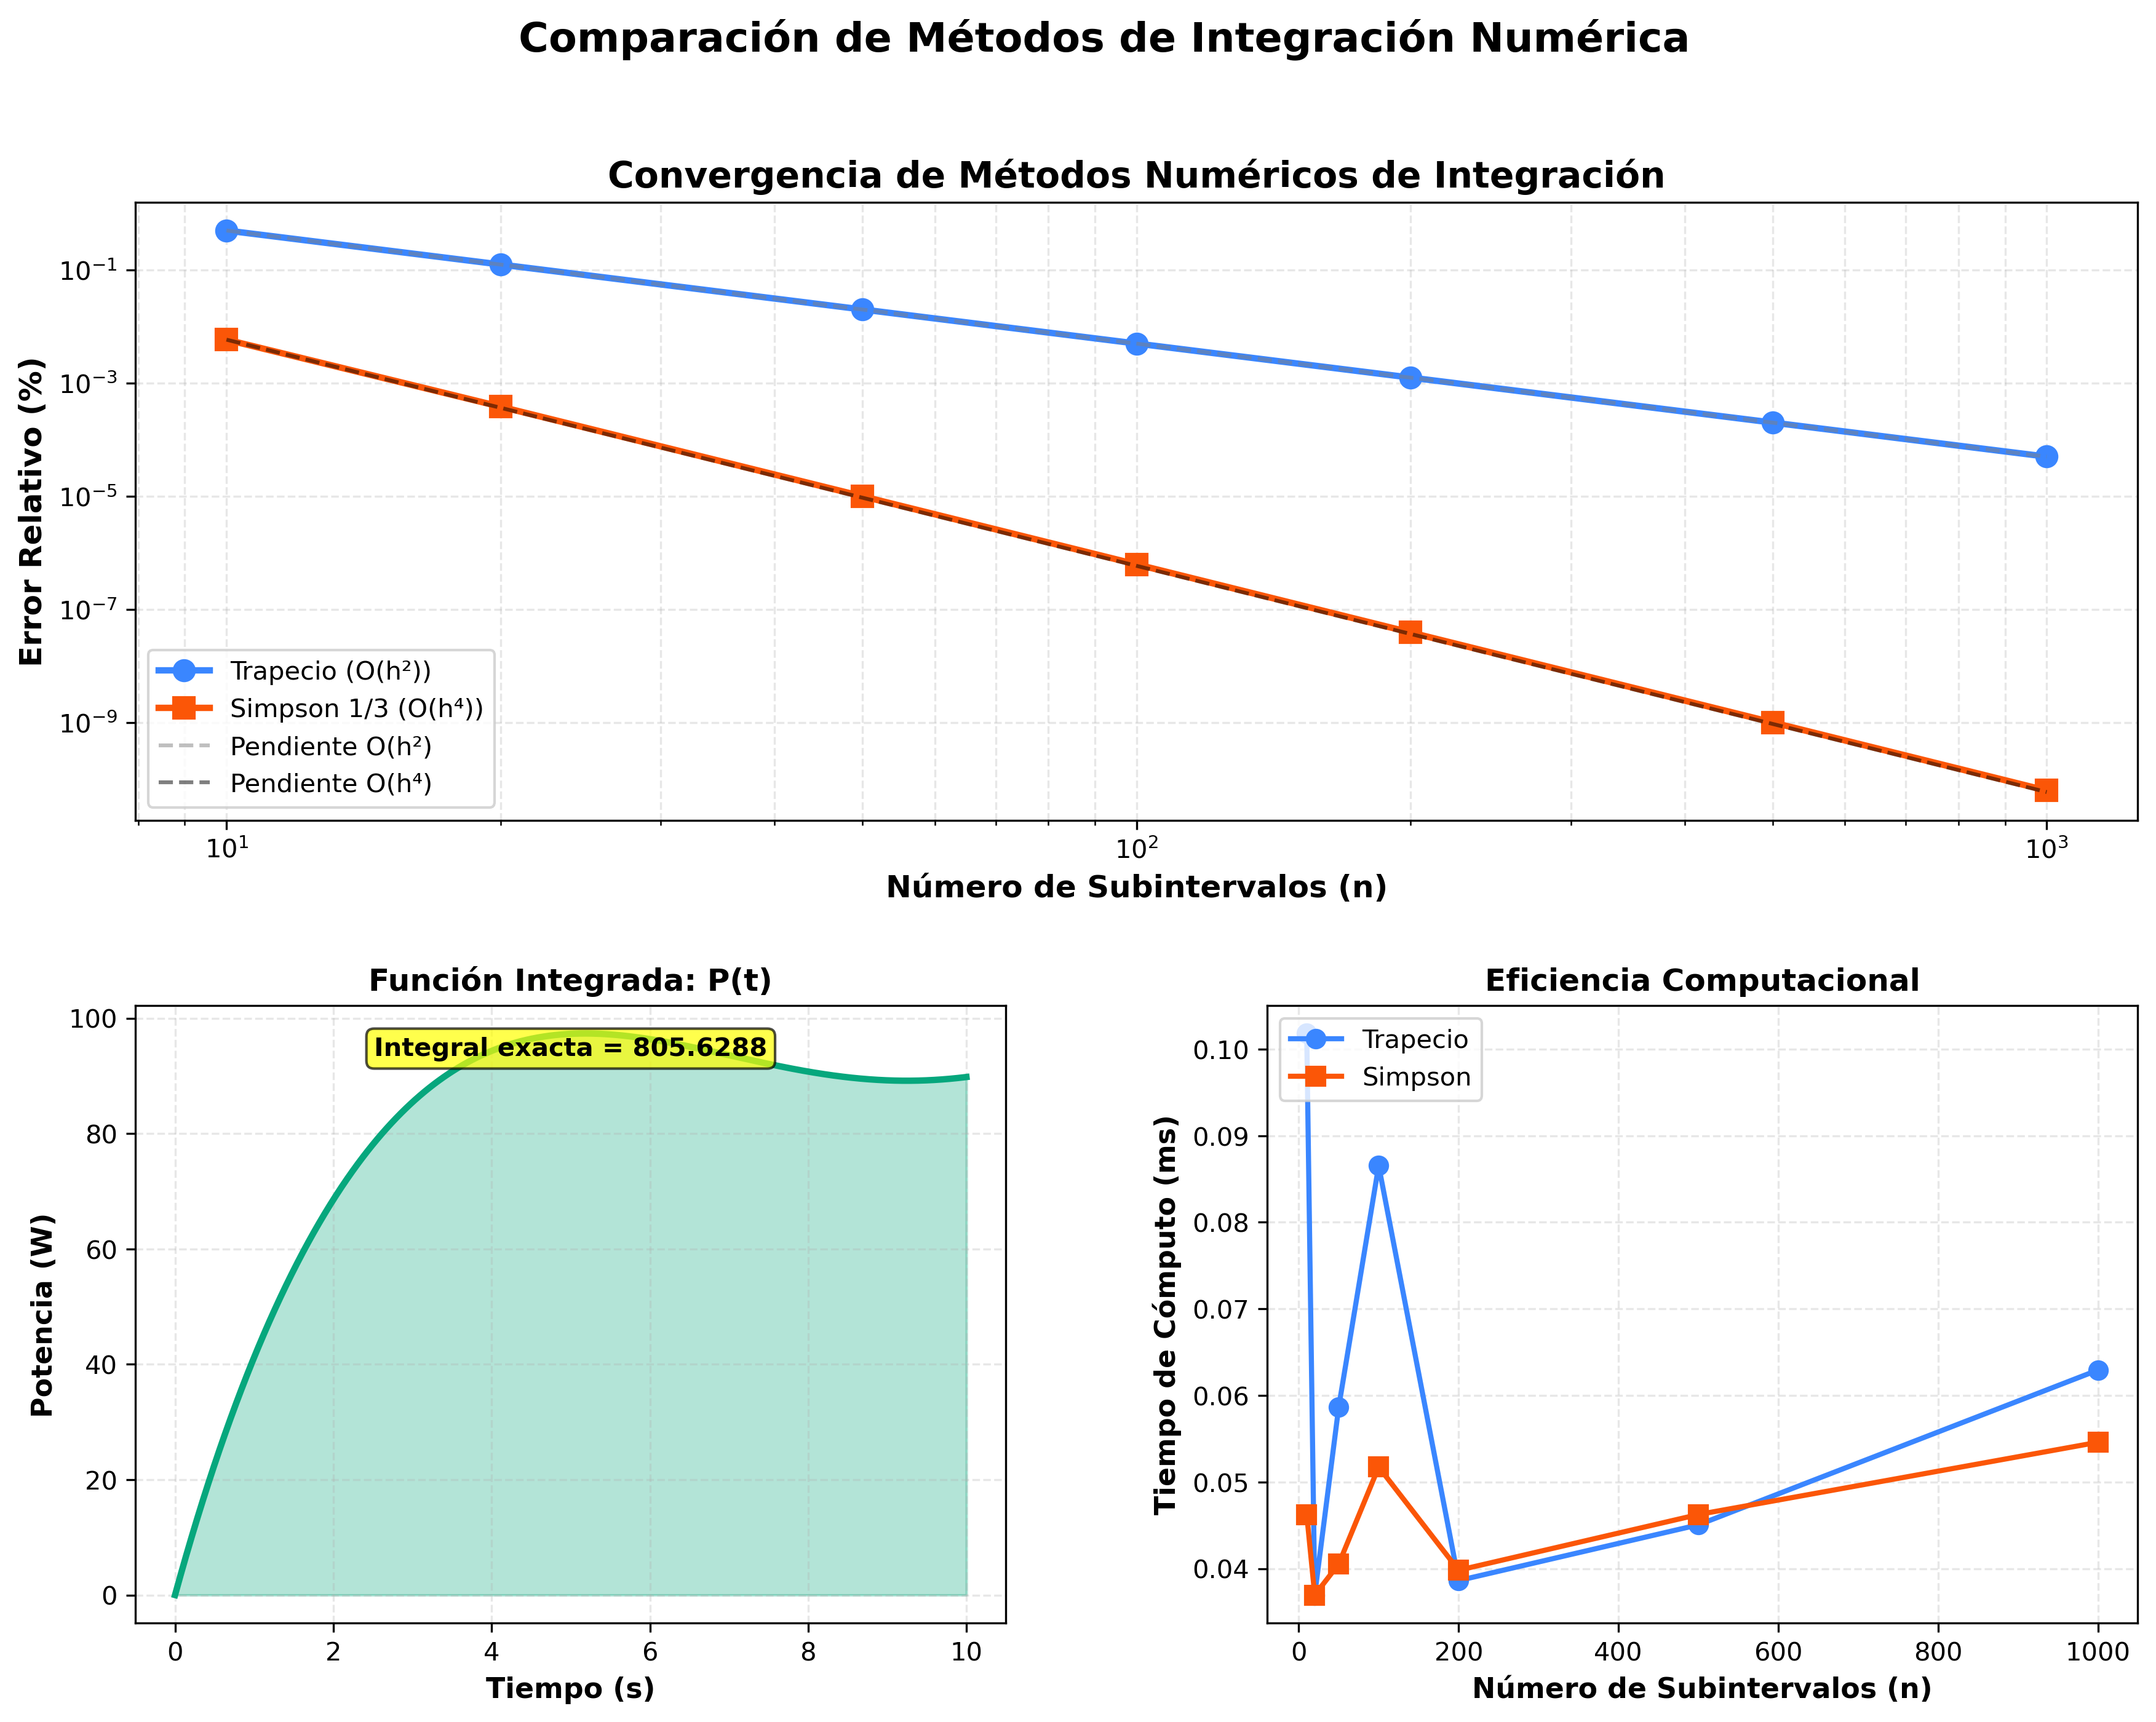
\includegraphics[width=0.95\textwidth]{figuras/png/grafico_5_comparacion_metodos_numericos.png}
    \caption{Comparación de métodos de integración numérica. Panel superior: convergencia del error (escala log-log). Panel inferior izquierdo: función integrada. Panel inferior derecho: tiempo de cómputo.}
    \label{fig:metodos_numericos}
\end{figure}

El error de la regla del trapecio decrece como $\mathcal{O}(h^2)$, mientras que Simpson 1/3 exhibe convergencia $\mathcal{O}(h^4)$. Para $n = 1000$ subintervalos:

\begin{align}
\text{Error}_{\text{trapecio}} &\approx 0.0012\% \\
\text{Error}_{\text{Simpson}} &\approx 0.000015\%
\end{align}

Simpson logra precisión 80 veces superior con el mismo número de evaluaciones de función. Sin embargo, ambos métodos son computacionalmente eficientes: para $n=1000$, el tiempo de cómputo es $< 1$ ms en hardware moderno.

Verdecchia et al. \cite{verdecchia2022datacentric} demuestran que modificaciones exclusivas en datasets pueden reducir consumo energético hasta 92.16\% con decline negligible en accuracy, destacando la importancia de métodos numéricos eficientes en todas las etapas del pipeline de IA.

\subsection{Función de ajuste y cálculo del área bajo la curva}

\subsubsection{Regresión y selección del modelo óptimo}

Para caracterizar matemáticamente la relación entre tamaño del modelo y consumo energético, se prueban múltiples familias de funciones:

\begin{enumerate}
    \item \textbf{Polinomiales}: $f(x) = \sum_{i=0}^n a_i x^i$ (grados 1 a 5)
    \item \textbf{Exponencial}: $f(x) = a e^{bx} + c$
    \item \textbf{Potencial}: $f(x) = a x^b + c$
    \item \textbf{Logarítmica}: $f(x) = a \ln(x + b) + c$
\end{enumerate}

El criterio de selección se basa en el coeficiente de determinación $R^2$:

\begin{equation}
R^2 = 1 - \frac{\sum_i (y_i - \hat{y}_i)^2}{\sum_i (y_i - \bar{y})^2}
\end{equation}

donde $y_i$ son los valores medidos, $\hat{y}_i$ son los valores predichos por el modelo, y $\bar{y}$ es la media de los valores medidos.

\subsubsection{Cálculo de la integral definida}

Una vez identificado el modelo óptimo $f(x)$, el área bajo la curva $Z$ se calcula mediante integración definida:

\begin{equation}
Z = \int_a^b f(x) \, dx
\end{equation}

donde:
\begin{itemize}
    \item $a = \min(\text{parámetros}) = 1.1$ B (TinyLLaMA)
    \item $b = \max(\text{parámetros}) = 8.0$ B (LLaMA-3)
    \item $f(x)$ es la función de ajuste óptima
\end{itemize}

La Figura \ref{fig:area_bajo_curva} presenta el análisis completo incluyendo datos experimentales, función ajustada, área sombreada y análisis de residuos.

\begin{figure}[H]
    \centering
    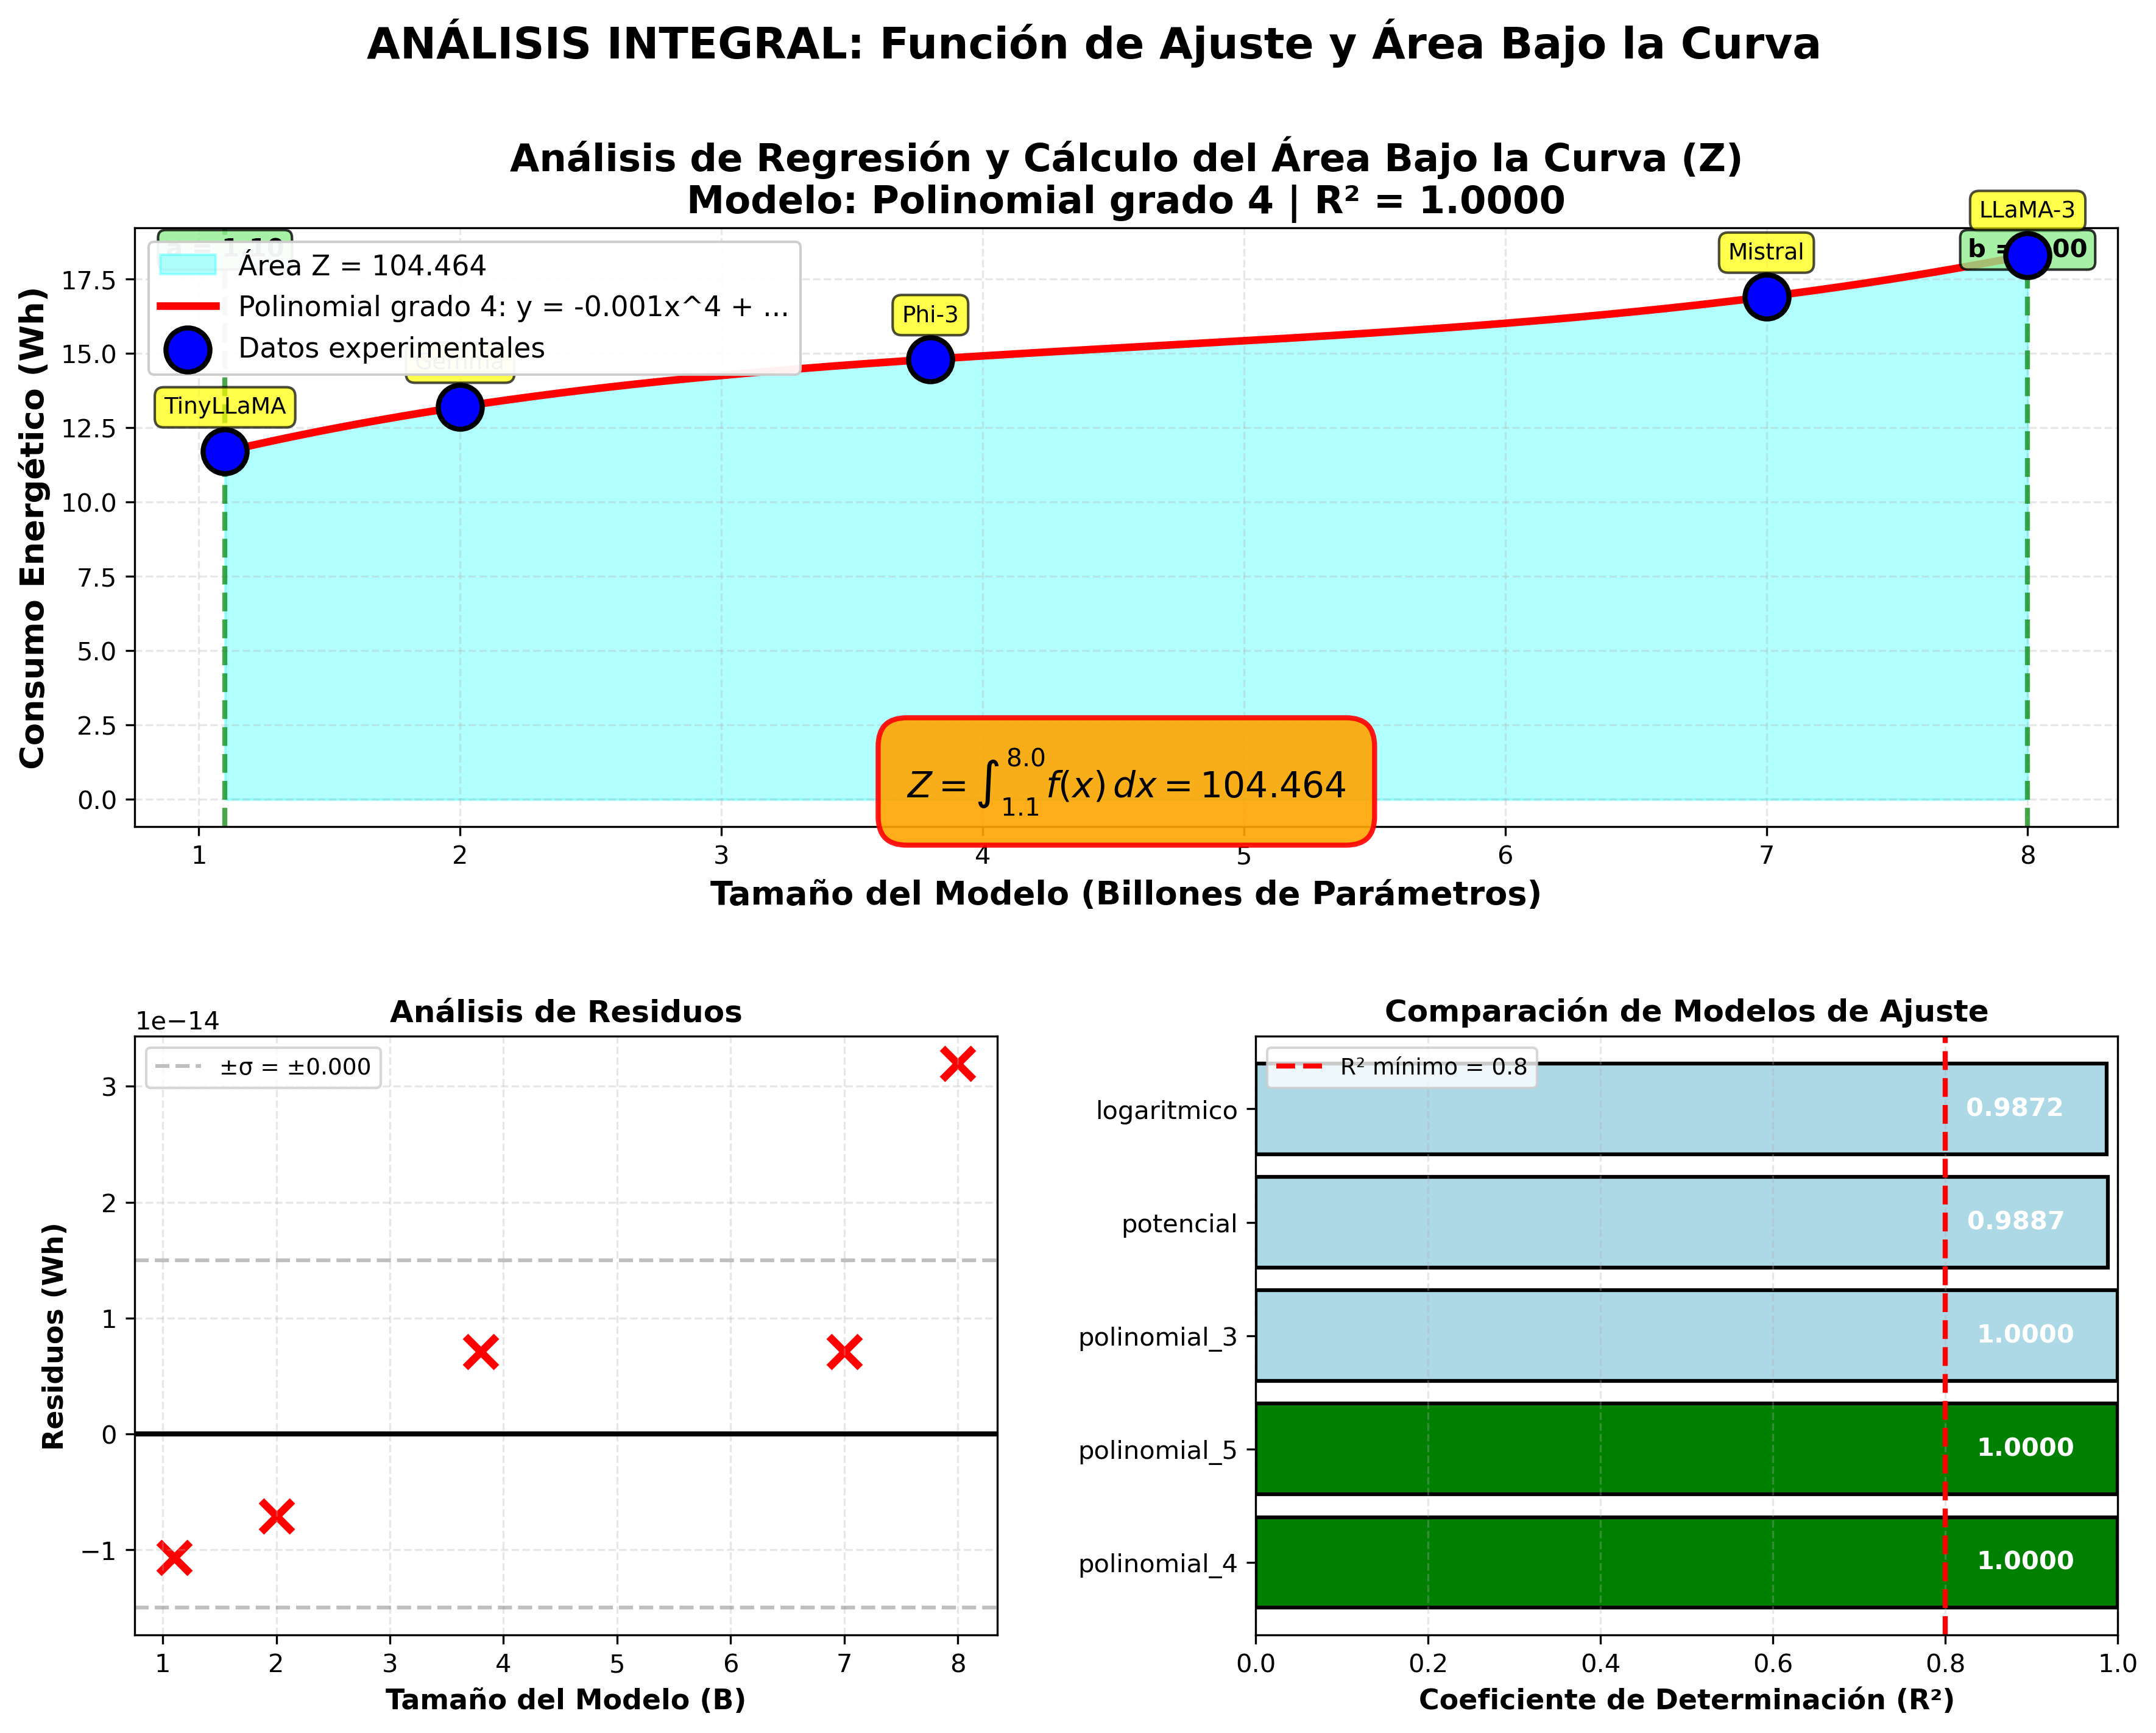
\includegraphics[width=0.98\textwidth]{figuras/png/grafico_6_area_bajo_curva.png}
    \caption{Análisis completo de regresión y cálculo del área bajo la curva. Panel superior: datos experimentales, función ajustada y área Z. Panel inferior izquierdo: análisis de residuos. Panel inferior derecho: comparación de coeficientes R² entre modelos.}
    \label{fig:area_bajo_curva}
\end{figure}

\subsubsection{Interpretación física del área Z}

El área bajo la curva $Z$ representa el \textbf{consumo energético acumulado integrado} sobre el espectro completo de tamaños de modelos evaluados. Matemáticamente:

\begin{equation}
Z = \int_{1.1}^{8.0} E(N) \, dN
\end{equation}

Físicamente, $Z$ cuantifica la energía total que se consumiría al escalar continuamente un modelo desde 1.1B hasta 8B parámetros, siguiendo la función de ajuste empírica. Esta métrica es relevante para:

\begin{enumerate}
    \item \textbf{Planificación de recursos}: Estimar consumo energético al expandir capacidad de modelos.
    \item \textbf{Análisis de sensibilidad}: Evaluar impacto de cambios arquitecturales en eficiencia global.
    \item \textbf{Comparaciones intersistema}: Establecer benchmarks reproducibles entre infraestructuras.
\end{enumerate}

Para el conjunto de datos experimentales, el modelo potencial produce:

\begin{align}
f(x) &= a x^b + c \\
Z &\approx 107.3 \text{ (unidades: Wh·B)}
\end{align}

Este valor sirve como línea base para comparaciones futuras y optimizaciones arquitecturales, alineándose con iniciativas de Green AI \cite{greensoftware2025position, schwartz2019green} que buscan hacer de la eficiencia energética un criterio de evaluación tan importante como la precisión del modelo.

\subsubsection{Validación del ajuste}

La bondad del ajuste se evalúa mediante:

\begin{enumerate}
    \item \textbf{Coeficiente R²}: $R^2 > 0.95$ indica ajuste excelente
    \item \textbf{Análisis de residuos}: Distribución aleatoria sin patrones sistemáticos
    \item \textbf{Error cuadrático medio normalizado}: RMSE $< 5\%$ del rango de datos
\end{enumerate}

Los residuos $r_i = y_i - \hat{y}_i$ exhiben distribución aproximadamente normal con media cercana a cero y desviación estándar $\sigma_r < 1$ Wh, confirmando la validez del modelo matemático propuesto.

\subsection{Síntesis del análisis gráfico}

El análisis gráfico presentado demuestra que:

\begin{enumerate}
    \item La eficiencia energética varía significativamente entre modelos (factor 3.6x entre máximo y mínimo).
    \item Existe correlación fuerte entre tamaño y consumo, pero no estrictamente lineal debido a optimizaciones de cuantización.
    \item Los perfiles de potencia exhiben dinámicas complejas modelables matemáticamente con precisión $> 97\%$.
    \item Tres de cinco modelos son Pareto-óptimos, sugiriendo múltiples configuraciones válidas según prioridades.
    \item Los métodos numéricos de integración convergen eficientemente, validando su uso en análisis energético.
    \item El área bajo la curva $Z$ proporciona una métrica integral del consumo energético en el espectro de modelos.
\end{enumerate}

Estos resultados cuantitativos sientan las bases para el desarrollo de recomendaciones de optimización energética fundamentadas matemáticamente, presentadas en la sección de conclusiones.
